%%%%%%%%%%%%%%%%%%%%%%%%%%%%%%%%%%%%%%%%%%%%

% formato FRONTE RETRO
\documentclass[epsfig,a4paper,11pt,titlepage,twoside,openany]{book}
\usepackage{epsfig}
\usepackage{plain}
\usepackage{setspace}
\usepackage[paperheight=29.7cm,paperwidth=21cm,outer=1.5cm,inner=2.5cm,top=2cm,bottom=2cm]{geometry} % per definizione layout
\usepackage{titlesec} % per formato custom dei titoli dei capitoli

\singlespacing

\usepackage[italian]{babel}

%%%%%%%%%%%%%%%%% STEFANO ADDED %%%%%%%%%%%%%%%%
% supporto lettere accentate
% queste due righe nel preambolo servono a poter utilizzare le lettere accentate in tutto il testo se no di norma si inserirebbero con \'e...
\usepackage[T1]{fontenc}
\usepackage[utf8]{inputenc}
\usepackage{hyperref} %Serve per i riferimenti
\usepackage{caption}  %Serve per le note (caption)
\usepackage{multicol}	 %Serve per usare più colonne

%%%%%%%%%%%%%%%%% ENRICO ADDED %%%%%%%%%%%%%%%%%
\usepackage{ulem} %Serve per il sottolineato
\usepackage{amsmath} %Serve per alcuni ambienti matematici
\usepackage{array} %Serve per le tabelle
\usepackage{multirow} %Seve per tabelle
\setcounter{secnumdepth}{5} %Utilissimo serve per aumentare il numero di paragrafi, si arriva fino a 5 livelli di profondità x.x.x.x.x
%GRAFICI
\usepackage{pgfplots}
\usepackage{pgfmath}
\usepackage{tikz}
%CODICE
% \usepackage{listings}
% \usepackage[cache=false]{minted} 
%\setminted{tabsize=4, breaklines, breakanywhere, linenos, mathescape,}

% \lstset{
% 	  breakatwhitespace=false,         
% 	  breaklines=true,     
% 	  basicstyle=\footnotesize\ttfamily,            
% 	  commentstyle=\color{blue}, %Indica il colore dei commenti
% 	  keywordstyle=\color{red}, %Indica il colore delle parole chiave
% 	  language=C, %Indica il linguaggio predefinito da usare
% 	  rulecolor=\color{black}, %Indica il colore dei numeri di righe
% 	  tabsize=4,
% 	  escapeinside={\%*}{*)},
% 	  morekeywords={}, %Altre parole da inserire tra le keywords. Ad esempio possiamo aggiungere do, gotttto, ecc ecc 
% }
%%%%%%%%%%%%%%%%% END OF ENRICO  %%%%%%%%%%%%%%%%

\begin{document}
%set the language of the text to italian
% !TeX spellcheck = it_IT

%%%%%%% personal commands (ALIAS):
% \newcommand{\nome_commando}[argomenti]{comando}
\newcommand{\e}[1]{$\cdot 10^{#1}$}
\newcommand{\mmax}[0]{mod\_withMax }
\newcommand{\mover}[0]{mod\_overlap }
\newcommand{\mmod}[0]{modularità modificata }
\newcommand{\nv}[0]{Node2Vec }
\newcommand{\wv}[0]{Word2Vec }
\newcommand{\cnrl}[0]{CNRL }
\newcommand{\cora}[0]{Cora }
\newcommand{\citeseer}[0]{Citeseer }
\newcommand{\LPred}[0]{Link Prediction }
%



%
%
\chapter{Implementazione}\label{chap:1}
In questo capitolo vengono spiegati i metodi utilizzati per cercare di migliorare le prestazioni dell'algoritmo di \cnrl \cite{CNRL_code}.
%
\section{Come funzionano le dinamiche di \cnrl}
In prima istanza vengono presi in input tutti i dati necessari, tra cui il grafo su cui si andrà a lavorare. Questo viene caricato in formato edgelist, ossia una lista d'archi identificati da una coppia nodo di partenza, nodo d'arrivo. Il grafo vien dunque preprocessato per utilizzare l'algoritmo \textbf{\nv} che effettuerà le visite. \nv\ è un algoritmo che regola le visite sulla base di due parametri $p$ e $q$. Questi due valori fanno variare l'esplorazione del grafo da una \textbf{visita in ampiezza (BFS)} ad una \textbf{visita in profondità (DFS)}, permettendo anche delle varianti intermedie.\\
I cammini individuati dalle visite effettuate con questo algoritmo sottostanno a ben definite caratteristiche. Da ogni nodo (in tutto $n$) partono $w$ cammini, per un totale di $w \cdot n$ cammini generati tutti di lunghezza al più $l$. È possibile che gli algoritmi non raggiungano la lunghezza $l$, in quanto il grafo è orientato ed è quindi possibile imbattersi in un pozzo. Si può immaginarlo come un vicolo cieco. In tali situazioni la visita si ferma, in quanto non è più possibile procedere, pertanto si avrà una lunghezza inferiore a $l$. Diversamente se si parla di grafi non orientati, tale problema non si pone poiché, anche se si arrivasse ad un pozzo, sarebbe sempre possibile tornare indietro, infatti \nv\ permette di ritornare su nodi già visitati.\\
\\
Ecco alcuni casi limite, perfettamente gestiti dall'algoritmo, che possono accadere durante la creazione dei cammini:
\begin{itemize}
	\item \textbf{nodo isolato su grafo orientato:} si avrà un cammino di lunghezza $1$, che comprende unicamente quel nodo
	\item \textbf{nodo isolato su grafo non orientato:} si avrà un cammino lungo $l$ contenente l'ID di quel nodo in continuazione
	\item \textbf{loop su grafo orientato:} questa è una sequenza di nodi che si ripete costante attraverso il cammino, è possibile iniziare con un nodo già presente nel loop o arrivarci dopo svariati passaggi
	\item \textbf{sequenze fisse finali su grafo orientato:} è possibile che tanti cammini terminino con la stessa sequenza di nodi. Questo accade perché sul grafo vi è un percorso senza possibilità di scelta che porta ad un pozzo: una volta imboccato tale percorso il cammino andrà a terminare sempre con la stessa sequenza
\end{itemize}
%
Una volta che \nv\ ha generato i cammini è compito di un'altra sezione ricavarne le comunità. Questo può essere fatto mediante due approci differenti. Il primo, il più noto, è \textbf{\wv} che va a considerare gli ID dei nodi come se fossero parole. La conseguenza è un cammino ossia un vettore di nodi che viene considerato come una sequenza di parole interpretabili come una frase. I dettagli del funzionamento si possono trovare nell'articolo "How exactly does word2vec work?"\cite{W2V_paper}.\\
Diversamente il codice di \cnrl\ utilizza, di default, un secondo metodo chiamato Latent Dirichlet Allocation (\textbf{LDA})\cite{LDA} o una sua variante detta \textbf{HalfLDA}. Entrambe le varianti si basano ancora su \wv. Le meccaniche esatte di questi metodi non erano di nostro interesse, pertanto non sono state e non verranno approfondite.\\
In questo caso non è rilevante quale algoritmo viene utilizzato, in quanto entrambi restituiscono un insieme di comunità, che formano la partizione cercata. Per dare una misurazione al lavoro svolto è ora possibile calcolare la modularità (spiegata in dettaglio nell'apposito capitolo sui metodi di valutazione).
%
\section{Introduzione degli attributi}
Per individuare le comunità esistenti \cnrl\ sfrutta unicamente la struttura del grafo.\\
Tuttavia entrambi i dataset su cui si è lavorato durante il tirocinio, denominati \cora\ e \citeseer\ (meglio spiegati nel capitolo sugli esperimenti), presentano oltre al file, che delinea la struttura del grafo, anche un secondo file, con estensione ".content", che contiene per ogni nodo una lista di valori binari, il cui significato è:
\begin{itemize}
	\item $0$ il nodo non ha l'attributo identificato da questa colonna
	\item $1$ il nodo ha l'attributo identificato da questa colonna
\end{itemize}
%
Tutte le informazioni contenute in questo file non sono considerate dal codice di \cnrl\ per questo motivo si è deciso d'introdurle. La finestra di codice, in cui è possibile apportare modifiche, è compresa fra il caricamento dei dati dall'input e l'inizio del processo d'estrazione delle comunità; ciò significa che la sola sezione in cui è possibile intervenire apportando delle modifiche è la generazione dei cammini lungo il grafo.\\
I cammini generati allo stato attuale non danno informazioni sugli attributi, pertanto è necessario, oltre a questi, aggiungerne altri che considerino tali informazioni. In particolare due nodi sono legati unicamente se vi è un arco che va da uno all'altro; intuitivamente si può dire che due nodi sono vicini e quindi legati se sono simili.\\
Questa somiglianza, se riportata sugli attributi, è possibile definirla: due nodi sono simili se condividono uno o più attributi, contrariamente non sono simili se non condividono nessun attributo. Data la definizione di somiglianza di due nodi attraverso gli attributi, si fa notare che vi è simmetria, pertanto verrà rappresentata attraverso un arco non orientato invece che uno orientato.\\
Si crea quindi un nuovo grafo indiretto che tiene conto di tutte le somiglianze derivanti dagli attributi, e su questo si richiama l'algoritmo di \nv\ per generare i nuovi cammini.
%
\section{Grafo degli attributi}
In questa sezione viene formalizzato il concetto di grafo degli attributi, una volta descritte le due alternative vengono esposti i necessari paragoni.\\
In partenza si rimuovono gli archi originari del grafo, poiché, se fossero inclusi, si rischierebbe di generare una seconda volta gli stessi cammini. Diversamente i nodi vanno conservati, in quanto sono questi i punti che si vogliono nuovamente collegare, da ora in avanti questo insieme di nodi prende il nome di \textbf{N1}.\\
Se due nodi condividono lo stesso attributo, sono simili e quindi connessi. Esistono tuttavia due metodologie per connettere i due nodi, $a$ e $b$: in maniera diretta o indiretta.
\begin{itemize}
	\item La maniera \textbf{diretta} consiste nel creare un arco non orientato (l'arco $(a, b)$) fra i due nodi; è il metodo più semplice
	\item La maniera \textbf{indiretta} consiste nel creare un nuovo nodo $c$, che verrà inserito nell'insieme \textbf{N2}, e creare due archi che collegano ogni nodo originario a $c$, quindi si creano i due archi $(a, c)$ e $(b, c)$.\\
	Questo metodo andrà a formare un nodo per ogni attributo esistente sul grafo, e andrà ad inserirli in N2
\end{itemize}
%
\begin{figure}[htp]
	\centering
	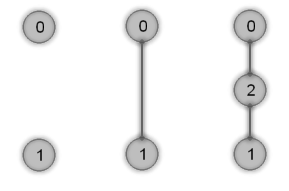
\includegraphics{immagini/add_att2}
	\caption{Due nodi condividono un attributo, ecco come possono essere legati, 1-nessun arco, 2-ipergrafo (completo), 3-grafo bipartito (a stella)}
	\label{fig:add_att2}
\end{figure}
\begin{figure}[htp]
	\centering
	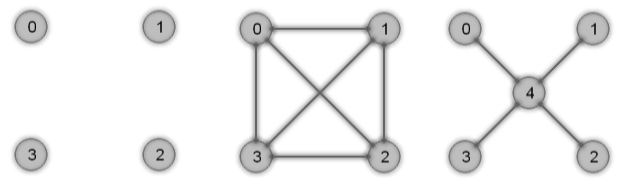
\includegraphics[width=\linewidth]{immagini/add_att4}
	\caption{Quattro nodi condividono un attributo, ecco come possono essere legati, 1-nessun arco, 2-ipergrafo (completo), 3-grafo bipartito (a stella)}
	\label{fig:add_att4}
\end{figure}
%
Nelle Figure~\ref{fig:add_att2} e~\ref{fig:add_att4} sono mostrati i due possibili metodi di collegamento dei nodi attraverso gli attributi. In ambedue le figure possiamo osservare tre scene:
\begin{enumerate}
	\item ci sono unicamente i nodi appartenenti all'insieme N1 a cui vanno aggiunti gli archi
	\item è mostrato il collegamento diretto. Da ogni punto raggiungo qualsiasi altro elemento attraversando esattamente un arco, ossia devo fare un singolo passo.\\
	Questa nuova struttura prende il nome di \textbf{ipergrafo}
	\item il collegamento è indiretto in quanto si passa attraverso il nodo $2$ in Figura~\ref{fig:add_att2} e attraverso il nodo $4$ in Figura~\ref{fig:add_att4}. Il nodo di collegamento è quello generato dagli attributi e pertanto apparterrà ad N2.\\
	Da ogni nodo di N1 è necessario utilizzare esattamente due passi per raggiungere un altro nodo di N1\\
	Questa nuova struttura prende il nome di \textbf{grafo bipartito}
\end{enumerate}
%
Si può notare come i due modelli siano molto differenti. Nella seconda parte viene creato un \textbf{grafo completo}, ciò sta ad indicare che il numero di archi presenti è altissimo poiché segue la legge binomiale $ \binom{n}{2}$ dove $n$ rappresenta il numero di nodi coinvolti.\\
Per il caso in Figura~\ref{fig:add_att4} vengono aggiunti $ \binom{4}{2} = 6$ archi, mentre il numero di nodi rimane invariato.\\
Diversamente nella terza parte viene costruito un \textbf{grafo a stella}. Vi è un nodo centrale che fa da fulcro per collegare tutti gli altri nodi. Questo comporta che vengano aggiunti $n=4$ archi e un nodo (Figura~\ref{fig:add_att4}).\\
\\
Dipendentemente dalla situazione si andrà a preferire un metodo piuttosto che l'altro: ecco le motivazioni che ci hanno guidati nella scelta.\\
Se vi sono tanti attributi e ognuno di questi appartiene ad un estremamente ristretto numero di nodi, allora ci si può permettere di creare degli ipergrafi. Diversamente, se ci sono anche pochi attributi che sono condivisi fra un alto numero di nodi, la scelta ricade sul grafo bipartito.\\
Un esempio di quest'ultimo caso è facile da trovare. Se esiste un attributo condiviso fra $100$ nodi questo significa che con il grafo bipartito andremo ad aggiungere un nodo e $100$ archi. Con l'ipergrafo non si aggiungerà nessun nodo ma in compenso bisogna creare $ \binom{100}{2} = 4950$ nuovi archi.\\
Situazioni come quella presentata in questo esempio sono state affrontate diverse volte durante il tirocinio. Per limitare il numero di archi su cui lavorare si è optato per il grafo bipartito.\\
\\
È importante far presente che quando si effettuano visite sul grafo bipartito si incontrano tutti i nuovi nodi dell'insieme N2, sconosciuti alle altre parti dell'algoritmo di \cnrl. Per questo motivo, una volta che \nv\ ha generato i cammini sul grafo, si deve rimuovere da ognuno di questi gli ID dei nuovi nodi generati, altrimenti nei futuri passaggi potrebbero verificarsi degli errori. Questo non sarebbe necessario se si fosse scelto l'ipergrafo, poiché non va a creare nessun nuovo nodo.
%
\subsection{Grafo bipartito e ipergrafo, origine dei nomi}
Si è parlato di ipergrafo e grafo bipartito senza però spiegarne le origini. Le Figure~\ref{fig:add_att2} e ~\ref{fig:add_att4} mostrano la situazione di alcuni nodi prendendo in considerazione un unico attributo. Tuttavia nei casi reali vi sono molti attributi. Ne consegue che entrambe le nuove strutture sono un insieme di tante piccole sezioni: il grafo bipartito è un insieme di grafi a stella e l'ipergrafo è un insieme di grafi completi.\\
Nel dettaglio:
%
\subsubsection*{Grafo bipartito}
Il grafo è detto bipartito in quando vi sono due insiemi di nodi, quelli che in precedenza son stati chiamati N1 (nodi originali) ed N2 (nodi derivanti dagli attributi). Tutti gli archi del grafo vanno da un nodo di N1 ad un nodo di N2 e viceversa visto che sono indiretti. Non esistono archi che vanno da N1 a N1 o da N2 a N2.\\
Questo è esattamente quello che ci si aspetta. Un arco da N1 ad N1 è un arco originario, quindi non necessita dell'attributo per passare da un punto ad un altro, poiché questi sono stati rimossi. Mentre un arco da N2 a N2 semplicemente non avrebbe significato, due attributi legati non hanno motivo d'esistere.
%
\subsubsection*{Ipergrafo}
Gli ipergrafi nella loro definizione formale non presentano semplici archi, ma dispongono di iperarchi. I normali archi possono essere rappresentati mediante una linea, poiché presentano due estremità entrambe legate ad un nodo. Diversamente gli iperarchi non possono essere rappresentati da una linea. Potrebbero arrivare ad avere infinite estremità, o meglio $n$ estremità dove $n$ è il numero di nodi nel grafo. Tutti i nodi che sono estremità di un iperarco possono raggiungere una qualsiasi delle altre estremità con un passo di lunghezza uno. Se si volesse rappresentare questa situazione su un grafo normale sarebbe necessario costruire un grafo completo per ogni iperarco.\\
È dunque chiaro il collegamento con la situazione presentata, ogni attributo altro non è che un iperarco. Nel nostro caso è stato necessario rappresentare gli iperarchi come archi normali in quanto l'algoritmo di \nv\ non è pensato per gestire la reale sintassi degli ipergrafi.
%
%
\section{Creazione del grafo - esempio}
In questa sezione viene mostrato come un grafo viene trasformato partendo dalla struttura di base fino a diventare un grafo bipartito o ipergrafo.\\
%
\begin{multicols}{2}
	\begin{center}
		\begin{tabular}{|c|cc|}
		\hline
		nodi&\multicolumn{2}{c|}{ID attributi}\\
		\hline
		1&11&\\
		2&11&12\\
		3&10&12\\
		4&11&13\\
		5&11&12\\
		6&12&13\\
		7&13&14\\
		\hline
		\end{tabular}
		\captionof{table}{Ad ogni nodo è associata la lista degli attributi che possiede}
		\label{tab:7_ID_to_att}
		%
		\begin{tabular}{|c|cccc|}
		\hline
		att&\multicolumn{4}{c|}{ID nodi}\\
		\hline
		10&3&&&\\
		11&1&2&4&5\\
		12&2&3&5&6\\
		13&4&6&7&\\
		14&7&&&\\
		\hline
		\end{tabular}
		\label{tab:7_att_to_ID}
		\captionof{table}{Ad ogni attributo è associata la lista dei nodi a cui appartiene}
	\end{center}
\end{multicols}
%
%
\begin{figure}[htp]
	\centering
	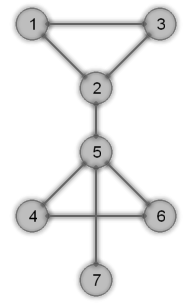
\includegraphics{immagini/7transform_str}
	\caption{Rappresentazione della struttura originaria del grafo}
	\label{fig:7transform_str}
\end{figure}
%
%
\noindent Nella Figura~\ref{fig:7transform_str} si vede la struttura del grafo di partenza.\\
Nella Tabella~\ref{tab:7_ID_to_att} si ha la lista di attributi che ogni nodo possiede.\\
Mentre la Tabella 2.2 %~\ref{tab:7_att_to_ID} TODO: perchè questo riferimento non funziona??
è inversa alla precedente (Tabella~\ref{tab:7_ID_to_att}) in quanto per ogni attributo sono mostrati tutti i nodi a cui appartiene.\\
Sono riportate entrambe le tabelle per comodità di comprensione, normalmente solo una è sufficiente.\\
Ecco come i due tipi di grafi vengono generati.
%
\begin{figure}[htp]
	\centering
	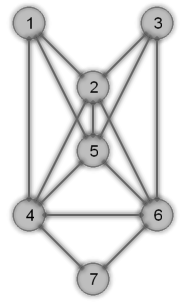
\includegraphics{immagini/7transform_hyper}
	\caption{Rappresentazione dell'ipergrafo generato}
	\label{fig:7transform_hyper}
\end{figure}
\\
Si osservi per primo l'ipergrafo mostrato in Figura~\ref{fig:7transform_hyper}.
\begin{itemize}
	\item  si può vedere come alcuni archi non sono più presenti. Due esempi sono $(1,3)$ e $(5,7)$, si ricorda che non sono questi due archi ad essere stati rimossi poiché tutti sono stati rimossi, semplicemente tutti gli altri sono stati nuovamente aggiunti diversamente da questi due
	\item  i nodi che condividono gli stessi attributi vanno a formare un grafo completo, due esempi sono $[1,2,4,5]$ con l'attributo $11$ e $[4,6,7]$ con l'attributo $13$
	\item  se solo un nodo dispone di un particolare attributo, nessun arco sarà creato. Questo è il caso dei due attributi $10$ e $14$.\\
	Questo può essere spiegato intuitivamente: si farebbe partire un arco da un nodo, ma questo non avrebbe mai una seconda estremità, e quindi non ha motivo d'esistere. O matematicamente: è un caso limite infatti $ \binom{1}{2} = error$ la linea numero $1$ del triangolo di tartaglia è $"1\ 1"$, non esiste il terzo elemento
\end{itemize}
%
\begin{figure}[htp]
	\centering
	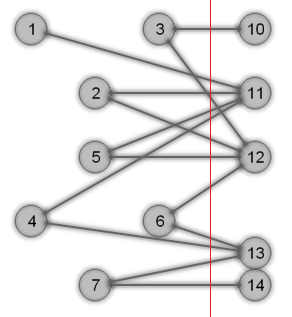
\includegraphics{immagini/7transform_bipartite}
	\caption{Rappresentazione del grafo bipartito generato}
	\label{fig:7transform_bipartite}
\end{figure}
%
Si osservi ora la più complessa situazione del grafo bipartito mostrato in Figura~\ref{fig:7transform_bipartite}. Non è facile capire cosa succede.\\
I nodi dall'1 al 7, sulla sinistra, sono i nodi originali, mentre i nodi dal 10 al 14 (maggiori o uguali a 10), sulla destra, sono i nuovi nodi generati dagli attributi.
\begin{itemize}
	\item i nodi sulla sinistra e sulla destra sono separati da un immaginaria linea verticale, e rappresentano i due insiemi di cui si parlava in precedenza, N1 e N2
	\item tutti gli archi attraversano la linea immaginaria, andando da sinistra a destra e viceversa
	\item tutti gli archi presenti nella struttura originaria di Figura~\ref{fig:7transform_str} non sono più presenti in quanto son stati rimossi e mai più rimpiazzati, perché non possono esistere archi da N1 a N1
	\item i nodi che condividono un attributo creano un grafo a stella, due esempi sono $[1,2,4,5]$ con l'attributo $11$ e $[4,6,7]$ con l'attributo $13$
	\item se solo un nodo possiede un particolare attributo questo non fa la differenza, i due attributi $10$ e $14$ sono comunque legati alla parte sinistra, come si può capire dalle tabelle
\end{itemize}
%\end{document}



